\chapter{Résultats}
Les expériences ont été réalisées avec Firefox 24.4.0 sur Linux à partir de différentes machines du pôle INGI \footnote{Pôle d'ingénierie informatique} de l'UCL. Elles ont été lancées via un terminal et Xvfb \footnote{Xvfb est un serveur X qui permet d'effectuer les opérations graphiques en mémoire.} était préalablement lancé, cela permet d'éviter des interactions fortuites entre le navigateur et l'utilisateur. Les dernières versions des extensions \textit{Firebug} et \textit{NetExport} disponibles au moment de chaque expérience étaient installées (à l'exception de l'expérience à long terme où l'ensemble des composants de l'expérience est resté stable).

\section{Expérience 1 : étude à long terme}
\subsection{Détails de l'expérience}
Le but de cette expérience est de déterminer l'évolution des trackers sur une certaine période en effectuant des mesures de façon régulière.

Afin de réaliser cette étude, le \textit{crawler} a été lancé chaque jour du 28 mars au 7 mai 2014 (à l'exception du 8 avril) sur le TOP 1000 du classement Alexa \cite{AlexaTop}, ce qui représente 40 jours de mesures. Notez cependant que l'implémentation du compteur de cookies Flash a été réalisée ultérieurement à cette expérience et ces données ne sont donc pas disponibles au sein de l'expérience.
\newline

Le \textit{crawler} a été lancé avec les paramètres suivants :
\begin{itemize}
	\item les sites visités sont issus du TOP Alexa du 26 mars 2014
	\item l'intervalle sélectionné concerne les 1000 premiers sites
	\item 3 tentatives maximum ont été autorisées par site
	\item Firefox était redémarré tous les 50 sites
	\item Firefox était dépourvu de toute extension (autre que Firebug et NetExport)
	\newline
\end{itemize}

\subsection{Premières constatations}
Le graphique de la \autoref{Exp1_crawler_fails} montre que l'efficacité du \textit{crawler} reste relativement stable tout au long de l'expérience car on peut voir qu'au maximum 90 sites sur 1000 sont en échec, soit un taux d'échec toujours inférieur à 9\%.
Notez que l'implémentation finale du \textit{crawler} a un peu changé depuis cette expérience. Lors de celle-ci, quand un site atteignait le nombre maximum de tentatives et qu'il était placé dans la liste des sites en échec, il était également retiré de la liste des sites ayant eu besoin d'au moins un nouvel essai suite à un timeout. Ceci explique des situations telles qu'au début du mois de mai où le nombre d'échecs est haut et le nombre de sites ayant été une fois en timeout est beaucoup plus bas.

\begin{figure}[!h]
	\centering
	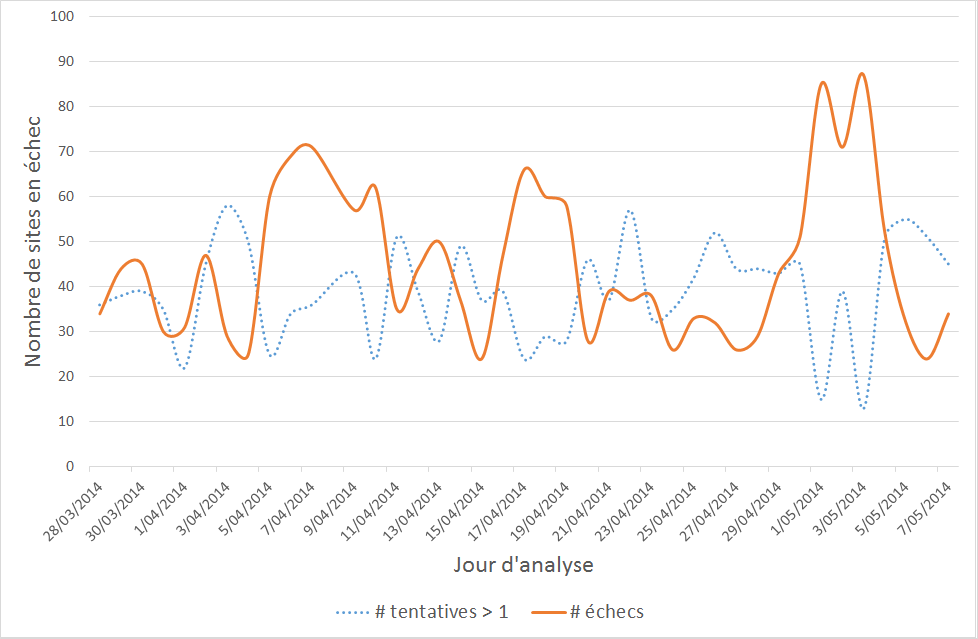
\includegraphics[scale=.6]{Exp_40jours/Exp1_crawler_fails.png}
	\caption{\label{Exp1_crawler_fails}Nombre de sites en échecs avec le \textit{crawler}.}
\end{figure}

La deuxième partie de l'expérience consistait à lancer le \textit{parser} afin d'analyser les fichiers générés lors du passage du \textit{crawler} sur les sites.
Le pourcentage de fichiers correctement analysés est représenté à la \autoref{Exp1_parser_success_rate}. On peut voir que du début de l'expérience jusqu'au 21 avril, le pourcentage de réussite est en moyenne de 99,73\%. A partir du 22 avril et jusqu'à la fin de l'expérience, il passe à 98,71\%, cela représente une dizaine de fichiers.
Croyant d'abord à une erreur lors de l'exécution du \textit{parser}, les analyses ont été reconduites une seconde fois mais n'ont pas montré de résultat différent.
Après analyse des fichiers de log du \textit{parser}, on remarque que ce sont généralement les mêmes sites qui sont en échec.
Ainsi, sur les 16 jours (du 22 avril jusqu'au 7 mai), on peut remarquer certains faits communs entre les analyses : une série de sites a rencontré des problèmes en même temps alors que d'autres n'ont été touchés que de manière temporaire.
\newline

\begin{figure}[!h]
	\centering
	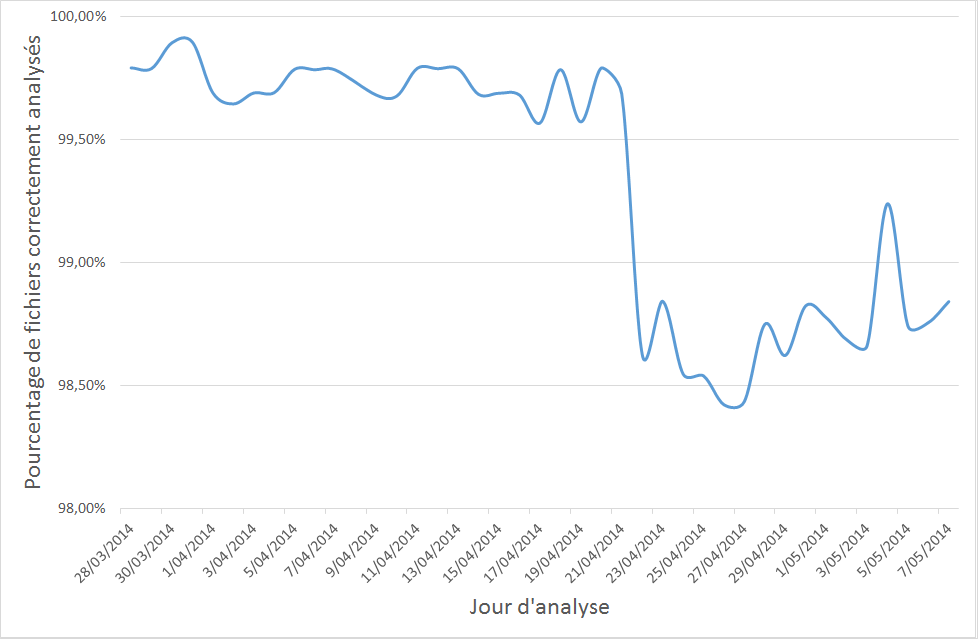
\includegraphics[scale=.6]{Exp_40jours/Exp1_parser_success_rate.png}
	\caption{\label{Exp1_parser_success_rate}Le pourcentage de réussite du \textit{parser}.}
\end{figure}

%Les sites suivants étaient chaque jour en échec:
%\begin{itemize}
%  \item 9gag.com
%  \item mashable.com
%  \item www.pixiv.net
%  \item www.wikihow.com
%  \newline
%\end{itemize}
%Les sites suivants n'ont pas été en échec 1 jour :
%\begin{itemize}
%  \item www.gamespot.com : le 4 mai
%  \item www.theverge.com : le 4 mai
%  \newline
%\end{itemize}
%Les sites suivants n'ont pas été en échec 2 jours :
%\begin{itemize}
%  \item www.thefreedictionary.com : le 25 avril et le 4 mai
%  \item www.wix.com : le 28 avril et le 4 mai
%  \newline
%\end{itemize}
%Les sites suivants ont été en échec sur une période de plusieurs jours :
%\begin{itemize}
%  \item www.rednet.cn : 3 jours (du 25 au 27 avril)
%  \item chinaz.com : 2 jours (les 27 et 28 avril)
%  \item www.groupon.com : 2 jours (les 5 et 6 mai)
%  \newline
%\end{itemize}
%Les sites suivants n'ont été en échec qu'un seul jour :
%\begin{itemize}
%  \item www.suning.com : le 22 avril
%  \item baomihua.com : le 24 avril
%  \item bleacherreport.com : le 26 avril
%  \item www.aili.com : le 27 avril
%  \item www.hm.com : le 30 avril
%  \item www.businessinsider.com : le 3 mai
%  \newline
%\end{itemize}
%Les autres sites en échec ne peuvent pas être classés de manière identique.\\

La constatation que certains sites sont en échec pendant la période complète des 16 jours (alors qu'ils ne l'étaient pas avant le 22 avril) et que certains sites sont en échec sur une courte période (2-3 jours) fait penser que ces échecs résultent d'une erreur située sur les sites eux-mêmes.

Une recherche approfondie a été effectuée et celle-ci a confirmé l'hypothèse selon laquelle l'erreur provient des données reçues des serveurs. Le \textit{parser} parcourt l'ensemble de chaque fichier HTTP Archive, celui-ci étant constitué de requêtes et réponses HTTP. La source des problèmes résulte d'une erreur dans certaines de ces réponses HTTP car elles ne respectent pas le standard défini par les RFC.
\\

Plus précisément, les erreurs proviennent de champs non reconnus dans les réponses HTTP ou de valeurs erronées.
Quelques exemples provenant des fichiers HTTP Archive ont été ajoutés afin d'illustrer les erreurs rencontrées.

\begin{figure}[h]
	\centering
	\lstinputlisting[style=dig]{examples/bad_field_google}
	\caption{\label{bad_field_google}Réponse HTTP de \textit{Google} et son cookie avec l'attribut "priority".}
\end{figure}
L'attribut \textit{priority} n'existe pas dans l'entête \textit{Set-Cookie} d'après la RFC 6265, section 5.2 \cite{IETF_RFC6265}. Or, on peut voir dans la \autoref{bad_field_google} que Google émet une réponse HTTP avec un tel attribut pour la création d'un cookie. Etant donné que l'utilisation des services de Google est fortement répandue, cette erreur a été constatée dans plusieurs fichiers HTTP Archive.

\begin{figure}[h]
	\centering
	\lstinputlisting[style=dig]{examples/bad_field_baidu}
	\caption{\label{bad_field_baidu}Réponse HTTP de \textit{Baidu} avec un attribut "domian".}
\end{figure}
Dans la \autoref{bad_field_baidu}, Baidu envoie une réponse HTTP qui contient une faute de frappe. En effet, au lieu de trouver un attribut "domain" (RFC 6265, section 5.2.3 \cite{IETF_RFC6265}), on constate la présence d'un attribut "domian". De plus, un autre attribut "domain" est déjà présent.
\newline

\begin{figure}[h]
	\centering
	\lstinputlisting[style=dig]{examples/bad_field_gamespot}
	\caption{\label{bad_field_gamespot}Réponse HTTP avec la valeur "0" pour l'attribut "expire".}
\end{figure}
Dans l'exemple de la figure \autoref{bad_field_gamespot}, on constate également un problème : la présence d'un attribut "expire" dans l'entête \textit{Set-Cookie} au lieu de "expires" (RFC 6265, section 5.2.1 \cite{IETF_RFC6265}). De plus, le format de date dans cet attribut est invalide.
\newline

Ces différents exemples montrent que la source des problèmes de traitement des fichiers HTTP Archive ne provient pas de l'implémentation du \textit{parser} mais provient plutôt d'erreurs dans les réponses HTTP reçues des serveurs.

\subsection{Nombre de trackers}
Le nombre total de trackers semble rester stable, il est en moyenne de 30080 (\autoref{Exp1_parser_total_trackers}). Ce nombre chute le 2 avril où il est de 25770 trackers. Ceci s'explique par le fait que le nombre de fichiers HTTP Archive pour ce jour (845 fichiers) est inférieur comparé aux autres jours, ce qui implique que moins de sites ont été analysés. Le nombre inférieur de fichiers provient probablement d'une perte de données suite à une suppression accidentelle ou à un manque d'espace disque qui a empêché l'enregistrement des fichiers HTTP Archive. L'export de ces fichiers étant externe à l'outil, celui-ci n'est pas en mesure de vérifier qu'ils sont correctement écrits sur le disque dur de la machine.

Des fluctuations dans le nombre total de trackers sont visibles car l'affichage des publicités sur les sites est généralement dynamique. Si une personne se rend sur une page puis la recharge, il est possible que les publicités soient différentes et proviennent d'autres régies publicitaires.

\begin{figure}[h]
	\centering
	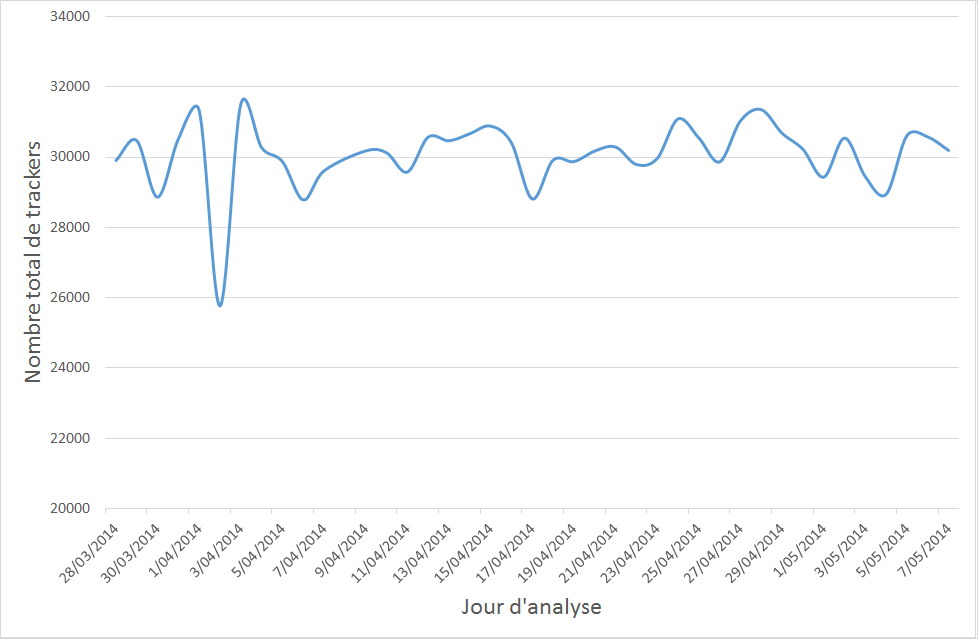
\includegraphics[scale=.56]{Exp_40jours/Exp1_parser_total_trackers.png}
	\caption{\label{Exp1_parser_total_trackers}Nombre total de trackers sur l'ensemble de l'analyse.}
\end{figure}

\newpage
\section{Expérience 2 : étude ponctuelle}
\label{experience_ponctuelle}
Cette expérience a été lancée de manière ponctuelle afin d'établir une image des sites à un instant donnée. Elle permet aussi de constituer la base de référence pour la comparaison des extensions.
\newline

Le \textit{crawler} a été lancé avec les paramètres suivants :
\begin{itemize}
	\item les sites visités sont issus du TOP Alexa du 16 mai 2014
	\item l'intervalle sélectionné concerne les 1000 premiers sites
	\item 3 tentatives maximum ont été autorisées par site
	\item Firefox était redémarré tous les 50 sites
	\item Firefox était dépourvu de toute extension (autre que Firebug et NetExport)
\end{itemize}

Les 36 sites suivants ont été en échec, ce qui signifie qu'aucun fichier HTTP Archive n'a été généré pour eux :
\begin{multicols}{3}
\begin{itemize}
  \item 39.net
  \item aili.com
  \item baomihua.com
  \item bitauto.com
  \item caijing.com.cn
  \item china.com
  \item csdn.net
  \item enet.com.cn
  \item gazeta.ru
  \item gmw.cn
  \item hao123.com
  \item heise.de
  \item howstuffworks.com
  \item ifeng.com
  \item ileehoo.com
  \item justdial.com
  \item kdnet.net
  \item lady8844.com
  \item microsoftonline.com
  \item moz.com
  \item online.sh.cn
  \item onlinesbi.com
  \item opensiteexplorer.org
  \item pchome.net
  \item people.com.cn
  \item pinimg.com
  \item qq.com
  \item secureserver.net
  \item sina.com.cn
  \item sohu.com
  \item tudou.com
  \item twimg.com
  \item yesky.com
  \item yoka.com
  \item youku.com
  \item zing.vn
\end{itemize}
\end{multicols}

Ces sites ne seront par conséquent pas analysés dans cette expérience.
\newline

Par ailleurs, 78 sites ont subi au moins un timeout mais ils ne seront pas listés ici. Notez que si ces sites ont rencontré 3 timeouts consécutifs, ils sont présents dans la liste des sites en échec (ci-dessus).
\newline

Le \textit{parser} a été lancé avec le paramètre suivant :
\begin{itemize}
	\item la base de données Ghostery utilisée est la version 303
	\newline
\end{itemize}

Le \textit{parser} n'a pas été en mesure d'analyser les fichiers suivants (les causes sont identiques à celles de l'expérience à long terme) :
\begin{multicols}{2}
\begin{itemize}
  \item 9gag.com.har
  \item accounts.google.com-2.har
  \item mashable.com.har
  \item website-unavailable.com-1.har
  \item www.babytree.com.har
  \item www.deezer.com.har
  \item www.gamespot.com.har
  \item www.gmail.com.har
  \item www.pixiv.net.har
  \item www.thefreedictionary.com.har
  \item www.theverge.com-1.har
  \item www.wikihow.com.har
  \item www.wix.com.har
\end{itemize}
\end{multicols}

Les sites correspondants à ces fichiers ne seront par conséquent pas analysés dans cette expérience.
\newline

L'analyse des fichiers HTTP Archive par le \textit{parser} a été effectuée deux fois : la première avec la base de données Ghostery et la seconde fois, sans cette base de données.

\subsection{Carte des trackers détectés}
La répartition des trackers par catégorie et pour les deux analyses est disponible aux Figures \ref{exp_normal_ghostery} et \ref{exp_normal_nog}.
%\newline

Concernant les cookies Flash, 79 sites ont créé au moins un fichier \textit{.sol}. Le site en ayant créé le plus (10 fichiers .sol) est \textit{espncricinfo.com}. En deuxième position, on trouve \textit{espn.go.com} avec 8 fichiers .sol créés lors de la visite du site. Les deux sites suivants sont \textit{nordstrom.com} et \textit{loading-delivery1.com} avec 4 fichiers .sol créés. Les 75 autres sites ont créé 3 cookies (9 sites), 2 cookies (9 sites) et 1 cookie (57 sites).

\subsubsection{Analyse avec la base de données Ghostery}
Comme on peut le constater sur la \autoref{exp_normal_ghostery}, la majorité des trackers détectés le sont par Ghostery (84\%). Ceci est normal car un premier tri est effectué avec l'aide de la base de données Ghostery. En deuxième position, viennent les URL externes appelées avec des paramètres (1350, soit 4,59\%) et en troisième position, les pixels de traçage de domaines tiers. Il apparaît qu'une partie non négligeable des pixels de traçage n'est pas détectée par Ghostery. Leur nombre est de 1212, ce qui représente 4,12\% de l'ensemble des trackers détectés par l'outil. Les codes JavaScript appelés avec des paramètres ont été détectés 1079 fois (3,67\%). Il y a également 888 réponses HTTP provenant de sites externes (3,02\%) qui créent un cookie tiers. Enfin, peu de fichiers Flash sont détectés par l'outil car ils représentent 0,84\% des éléments détectés, soit 246 éléments. Au total, 29402 trackers ont donc été détectés.

\begin{figure}[!h]
	\centering
	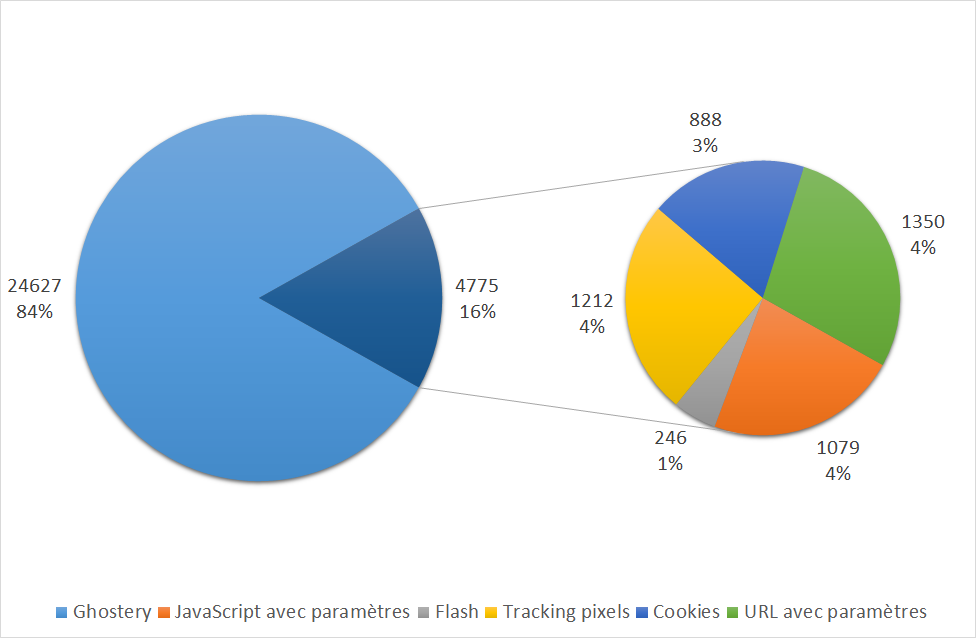
\includegraphics[scale=.6]{resultats/ANALYSES/Images/Normal-Ghostery.png}
	\caption{\label{exp_normal_ghostery}Répartition des trackers par catégorie (avec Ghostery).}
\end{figure}

\begin{figure}[!h]
	\centering
	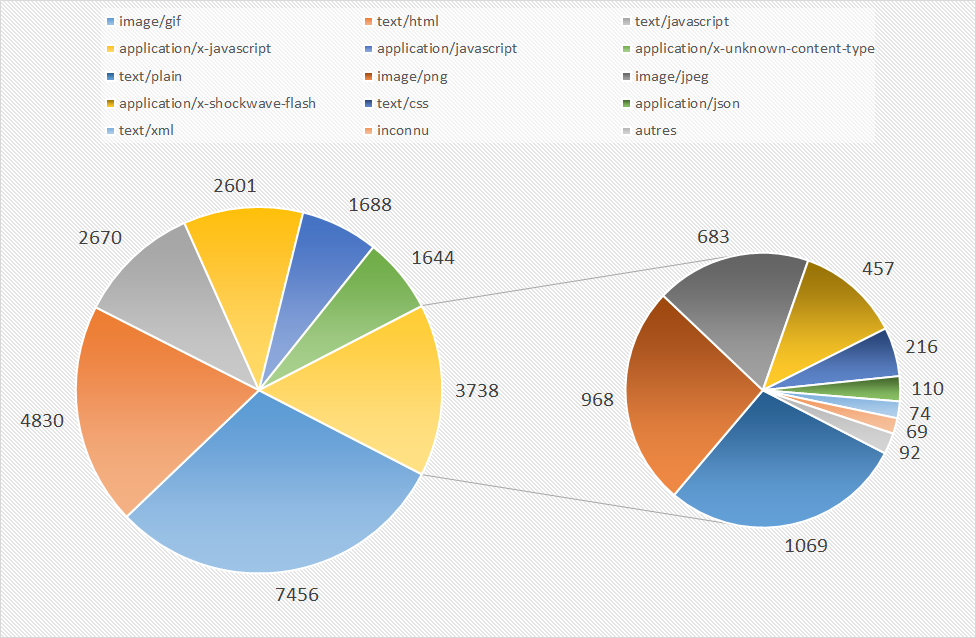
\includegraphics[scale=.6]{resultats/ANALYSES/Images/Normal-Ghostery-mimetype.png}
	\caption{\label{exp_normal_ghostery_mimetype}Répartition des types de trackers détectés par Ghostery.}
\end{figure}

\begin{figure}[!h]
	\centering
	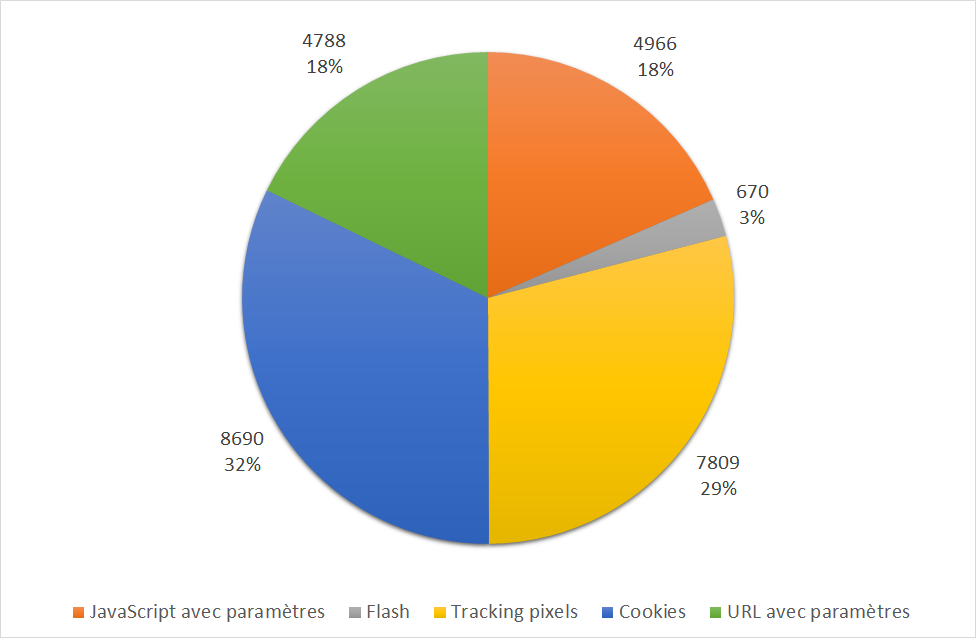
\includegraphics[scale=.6]{resultats/ANALYSES/Images/Normal-NoG.png}
	\caption{\label{exp_normal_nog}Répartition des trackers par catégorie (sans Ghostery).}
\end{figure}

Lorsqu'une ressource est détectée comme étant un tracker par Ghostery, le \textit{parser} enregistre le type de cette ressource (voir des exemples dans l'Annexe \ref{ghostery_mimetypes}). Les résultats sont visibles à la \autoref{exp_normal_ghostery_mimetype}. Ils montrent que le premier type de trackers est de type \textit{.gif} (7456 trackers). La deuxième position est occupée par le JavaScript (si on rassemble \textit{text/javascript}, \textit{application/x-javascript} et \textit{application/javascript}) avec 6959 trackers et la troisième position concerne les ressources de type "text/html".

Ceci montre que les principaux trackers importés de sites tiers sont les pixels de traçage ainsi que les codes écrits en JavaScript.
%\newline

Au vu des deux graphiques (Figures \ref{exp_normal_ghostery} et \ref{exp_normal_ghostery_mimetype}), l'origine principale des trackers est la présence d'images \textit{.gif} jouant le rôle de pixels de tracking et de l'inclusion de codes JavaScript. Ces trackers représentent la majorité des éléments détectés par Ghostery et ils sont respectivement au nombre de 1212 et 1079 d'après les critères opérant après le premier tri effectué par Ghostery.

\subsubsection{Analyse sans la base de données Ghostery}
La \autoref{exp_normal_nog} reprend l'ensemble des trackers détectés lors de l'analyse effectuée sans la prise en compte de la base de données Ghostery. Pour rappel, seuls les éléments chargés depuis un domaine tiers sont présents dans ce graphique.

La plus grande portion du graphique (32,28\%) se compose des créations de cookies tiers. La seconde (29\%) est constituée des pixels de traçage et le trio de tête se termine par les codes JavaScript chargés avec des paramètres (18,45\%). Les URL appelées avec des paramètres sont juste derrière avec 17,78\% des trackers détectés et les fichiers Flash représentent (2,49\%). Au total, 26923 trackers ont été repérés.

\subsection{Discussion sur les résultats des deux types d'analyse}
\label{discussion_analyses}
On remarque que le nombre de trackers détectés est plus élevé pour l'analyse ayant utilisé la base de données Ghostery (29402 contre 26923).
Ceci s'explique par plusieurs raisons.
\newline

La première est que les images issues de domaines tiers et connues comme étant des trackers sont détectées par Ghostery mais ne le sont pas par les autres critères. Une telle détection n'est pas envisageable sans l'aide d'une base de données car il est impossible de savoir ce qu'il se passe du côté du serveur. Par contre, les pixels espions sont détectés grâce à leur particularité.
\newline
\newpage

La seconde raison porte sur les codes JavaScript. Seuls les codes JavaScript appelés avec une requête HTTP dont l'URI possède une chaîne de requête sont considérés comme des trackers par les critères définis. Il existe également des trackers JavaScript qui n'ont pas de chaîne de requête mais les considérer systématiquement comme des trackers provoquerait beaucoup de faux positifs. La solution idéale serait d'analyser le comportement de ces scripts afin de déterminer si ce sont des trackers ou non.
\newline

A l'inverse, le nombre de trackers détectés par l'analyse n'utilisant pas la base de données Ghostery peut parfois être supérieur dans certaines catégories. En effet, les critères retiennent toutes les ressources Flash et les URL possédant un champ de requête. Cependant, tous ces éléments ne sont pas des trackers même si force est de constater que la plupart en sont.
\newline

L'utilisation d'une base de données permet de détecter des éléments qui ne seraient pas suspectés d'être des trackers. Cependant, elle peut également passer à côté de trackers qui ne sont pas renseignés dans cette base.

Cela est d'ailleurs flagrant avec la détection des pixels espions. Malgré l'utilisation de la base de données Ghostery, 1212 pixels de traçage ont été détectés par les critères définis au sein du \textit{parser}.
\newline

Chaque analyse a ses avantages et ses inconvénients : celle qui n'utiliserait que la base de données Ghostery aurait peu (voire pas) de faux positifs mais passe à côté de certains trackers absents de sa base de données alors que l'analyse n'utilisant pas cette base peut renfermer plus de faux positifs mais détecte aussi plus de trackers de certaines catégories.
\newline

L'outil développé pour ce mémoire propose deux types d'analyses : le premier utilise la base de données Ghostery et applique les critères définis sur les ressources n'ayant pas été détectées par la base de données. Le second ne repose que sur les critères définis.

Un expérimentateur choisissant le premier type d'analyse bénéficiera donc des avantages de l'utilisation de la base de données mais également des critères définis.
\newpage

\subsection{Sites renfermant le plus de trackers détectés}
Le TOP 10 des sites en nombre de trackers détectés pour les deux analyses sont :\\

\begin{tabular}{ c | p{5cm} | c || p{5cm} | c | }
   Rang & Avec la base Ghostery & \# & Sans la base Ghostery & \# \\
   \hline
   1 & drudgereport.com & 341 & drudgereport.com & 385\\
   2 & www.hongkiat.com & 333 & www.primewire.ag & 367\\
   3 & www.primewire.ag & 284 & www.hongkiat.com & 364\\
   4 & www.theblaze.com & 256 & www.theblaze.com & 332\\
   5 & photobucket.com & 240 & photobucket.com & 280\\
   6 & slickdeals.net & 226 & www.jeuxvideo.com & 271\\
   7 & www.linternaute.com & 223 & tinypic.com & 268\\
   8 & www.jeuxvideo.com & 213 & slickdeals.net & 248\\
   9 & www.engadget.com & 209 & www.linternaute.com & 240\\
   10 & tinypic.com & 201 & www.commentcamarche.net & 235\\
   \hline
\end{tabular}
\newline

Les deux analyses rapportent des résultats similaires pour la désignation des 10 sites renfermant le plus de trackers à l'exception de \textit{www.engadget.com} qui se trouve seulement dans le TOP 10 de l'analyse utilisant la base de données Ghostery et \textit{www.commentcamarche.net} qui se trouve seulement dans le TOP 10 de l'autre analyse qui n'utilise pas la base de données de trackers.

\subsection{Organisations déployant le plus de trackers}
Selon cette analyse, en ne considérant que les trackers détectés par Ghostery, voici la liste des organisations qui en génèrent le plus.\\
%\newline
Sur un total de 24626 trackers :
\begin{multicols}{2}
\begin{itemize}
  \item 2562 : DoubleClick
  \item 1379 : AppNexus
  \item 949 : Google Analytics
  \item 675 : Google Adsense
  \item 574 : Rubicon
  \item 534 : Turn
  \item 441 : ScoreCard Research Beacon
  \item 347 : MediaMath
  \item 332 : Lotame
  \item 326 : OpenX
\end{itemize}
\end{multicols}

Quand on sait que \textit{DoubleClick} appartient à \textit{Google}, cela fait 4856 trackers provenant du géant mondial. Cela représente un peu moins de 20\% des trackers détectés au total par la base de données Ghostery. Le second est \textit{AppNexus} avec 5,60\% (1379 trackers), il s'agit d'une plateforme fonctionnant sous le modèle RDB \footnote{RDB (Real Time Bidding) est un système qui permet à des annonceurs de placer leurs publicités selon un système d'enchères. Il repose sur une plateforme d'achat et vente de publicités en temps réel.}.
\\
Ensuite, on trouve Facebook et Adobe quasiment ex \ae{}quo avec respectivement 2,81\% (691 trackers) et 2,78\% (685 trackers). Pour terminer, il y a 2 autres entreprises au dessus de la barre des 2\%, 7 entreprises entre 1 et 2\% et les autres (plus de 500 entreprises) avec un pourcentage inférieur à 1\%.
\newline

Il faut également noter qu'AppNexus utilise différents services dont principalement ceux de Google (en 2010, il semblerait que Google comptait pour 50\% \footnote{D'après un expert de l'industrie publicitaire (\url{http://techcrunch.com/2010/11/30/google-temporarily-blocks-appnexus-from-its-ad-exchange/})}). Il est donc possible que cela permette à Google d'amasser encore plus de statistiques grâce à cet intermédiaire. Cette répartition montre que de grands groupes tracent massivement les utilisateurs mais qu'il existe énormément de petites entreprises qui tracent également les utilisateurs mais dans une moindre mesure. 
